\documentclass[a4paper]{article}

%% Language and font encodings
\usepackage[english]{babel}
\usepackage[utf8x]{inputenc}
\usepackage[T1]{fontenc}
\usepackage{graphicx}
\usepackage{caption}
\usepackage{subcaption}
\usepackage{eurosym}
\usepackage{multirow}
\usepackage{footnote}
\usepackage{listings}
\usepackage{color}
\usepackage{pdfpages}

%% Sets page size and margins
\usepackage[a4paper,top=3cm,bottom=2cm,left=3cm,right=3cm,marginparwidth=1.75cm]{geometry}

%% Useful packages
\usepackage{amsmath}
\usepackage{graphicx}
\usepackage[colorinlistoftodos]{todonotes}
\usepackage[colorlinks=true, allcolors=blue]{hyperref}
\begin{document}

\begin{titlepage}

\newcommand{\HRule}{\rule{\linewidth}{0.5mm}} % Defines a new command for the horizontal lines, change thickness here

\center % Center everything on the page
 
%----------------------------------------------------------------------------------------
%	HEADING SECTIONS
%----------------------------------------------------------------------------------------

\textsc{\LARGE Ecole Polytechnique de Bruxelles}\\[1.5cm] % Name of your university/college
\textsc{\LARGE University of Leeds}\\[1.5cm]
\textsc{\large Johnston Lab Internship}\\[0.5cm] % Minor heading such as course title

%----------------------------------------------------------------------------------------
%	TITLE SECTION
%----------------------------------------------------------------------------------------

\HRule \\[0.4cm]
{ \huge \bfseries User Guide Lick Sensor}\\[0.4cm] % Title of your document
\HRule \\[1.5cm]
 
%----------------------------------------------------------------------------------------
%	AUTHOR SECTION
%----------------------------------------------------------------------------------------

\begin{minipage}{0.4\textwidth}
\begin{flushleft} \large
\emph{Author:}\\
Maxime \textsc{Verstraeten} % Your name
\end{flushleft}
\end{minipage}
~
\begin{minipage}{0.4\textwidth}
\begin{flushright} \large
\emph{Supervisor:} \\
Jamie \textsc{Johnston}\\[0.3cm] % Supervisor's Name
\end{flushright}
\end{minipage}\\[2cm]

% If you don't want a supervisor, uncomment the two lines below and remove the section above
%\Large \emph{Author:}\\
%John \textsc{Smith}\\[3cm] % Your name

%----------------------------------------------------------------------------------------
%	DATE SECTION
%----------------------------------------------------------------------------------------

{\large \today}\\[2cm] % Date, change the \today to a set date if you want to be precise

%----------------------------------------------------------------------------------------

\vfill % Fill the rest of the page with whitespace

\end{titlepage}


\noindent\rule{\textwidth}{1pt}

\tableofcontents

\newpage

\listoffigures

\newpage



\section{Introduction}
This user guide intends to provide the user with the information required to use and understand the lick-sensor device developed at JohnstonLab as well as giving some clues regarding troubleshooting.


\section{Objective}
The lick-sensor device is intended to be use for mice behavioral studies in a kind of reward system with sugared water. The device allows a mouse to lick a needle which shall deliver some water through a valve. The amount delivered can be setup logically with an Arduino code as well as the conditions required for delivery (e.g. the minimum delay between two deliveries, in case of specific odors delivered, ...). 

\section{Hardware}
\subsection{Water Tank}
The water should be stored higher than the delivery as to provide pressure for the water to flow through the valve.
\subsection{Valve}
The chosen valve is a solenoid valve VDW22LA for its size, price and speed of actuation. It is working with 24V DC and as it is a solenoid valve, will create peak voltage and current when switching it off/on.
\subsection{Enclosure}
The device comes with its enclosure which implements a switch, a push-button as well as a BNC input for valve activation, 4 BNC connectors (24V valve, GND valve, sensor+, sensor -), a 9V output for the fan and 2 BNC outputs for the licking signal and the valve activation signal.
\subsection{Fan}
Because of the use of linear voltage regulators (at least in early designs), a fan had to be added to the enclosure. It is a simple fan MC002111 working on max 12V DC.

\subsection{Microcontroller}
The µC used is an Arduino Uno. The PCB is designed to be stacked on top of it so that each PCB pin is correctly connected to the Arduino. 

\section{Software}
The Arduino has been programmed using Arduino IDE. 

It works around interrupts being polled every loop.
The sensor circuit, once powered, is able to output 3.3V TTL output to pin 2. Once a change is detected, an interrupt is triggered which sets a flag to True. In the loop, the flag will be reset and, if the conditions are met, an appropriate duration output is set to pin 6. This 3.3V signal will then be sent to another reed relay functioning with 24V. This will therefore activate the valve for the specific duration.

It works the same way for the switch, push-button and BNC input.

\section{How to use?}
The device is simple to use.

It should be powered through the DC socket with a 24V DC supply. The bullet connectors shall be connected to the crocodile clamps of the sensor and the bullet connectors of the valve. Obviously, correct polarity must be observed for the valve.
If the device is overheating (which it should not with the new DC switching regulator), you can power the fan by connecting the two battery plugs.

The valve is activated when both sensors are touched at the same time or when the push-button is pressed or the switch is in up position.

\section{Expected Results}
The valve should open briefly when the two sensors are touched or when the push-button is pressed.
\section{Electronic Circuits}
\subsection{Sensor circuit}
The basic sensor circuit is based of a paper (Slotnick, A simple 2-transistor touch or lick detector circuit, 2009) and allows to send a TTL output whenever an animal touches two wires at the same time.

\begin{figure}[h!]
    \centering
    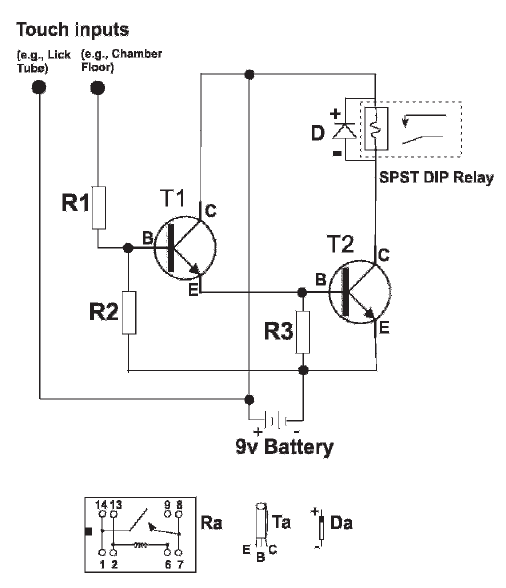
\includegraphics[width = 10cm]{images/sensor.png}
    \caption{Sensor circuit}
    \label{fig:sensor}
\end{figure}

It is obvious that since the animal subject must survive the experiment and ideally not notice the lick sensor, the current flowing through the rodent should be minimal..
A battery-operated circuit makes it independent from a DC power supply and an AC line and thus does not require isolation transformer (or optocoupler, ...) to protect the rodent.

The circuit proposed here above is using a 9V battery, the current flowing is less than 1µA and the output operates a relay that can then act as a switch to operate any microcontroller, whatever the voltage required for the logic inputs and therefore not requires level shifting (directly outputs TTL-compatible pulses)

According to the paper, a 9V alkaline battery is sufficient for a couple of months of experiment. 5.5V is the minimum battery voltage for reliable operation. A 9V lithium battery could have an extended lifetime.

The battery could also be replaced by a Zener in 6.3V from a 12 or 24V DC power supply which allows unlimited lifetime and controlled voltage. This should only be done in case of sustained contact. Otherwise, probably a million operations before the battery is drained out.

\subsection{Actual implementation}
The sensor circuit is only a small part of the whole circuit. Moreover, I decided to add a pull-down at the output of the TTL relay and add some decoupling capacitors on the circuit.
The BJTs used are PN2222A and the relays are COTO 9007-05-01 SPST.

\begin{figure}[h!]
    \centering
    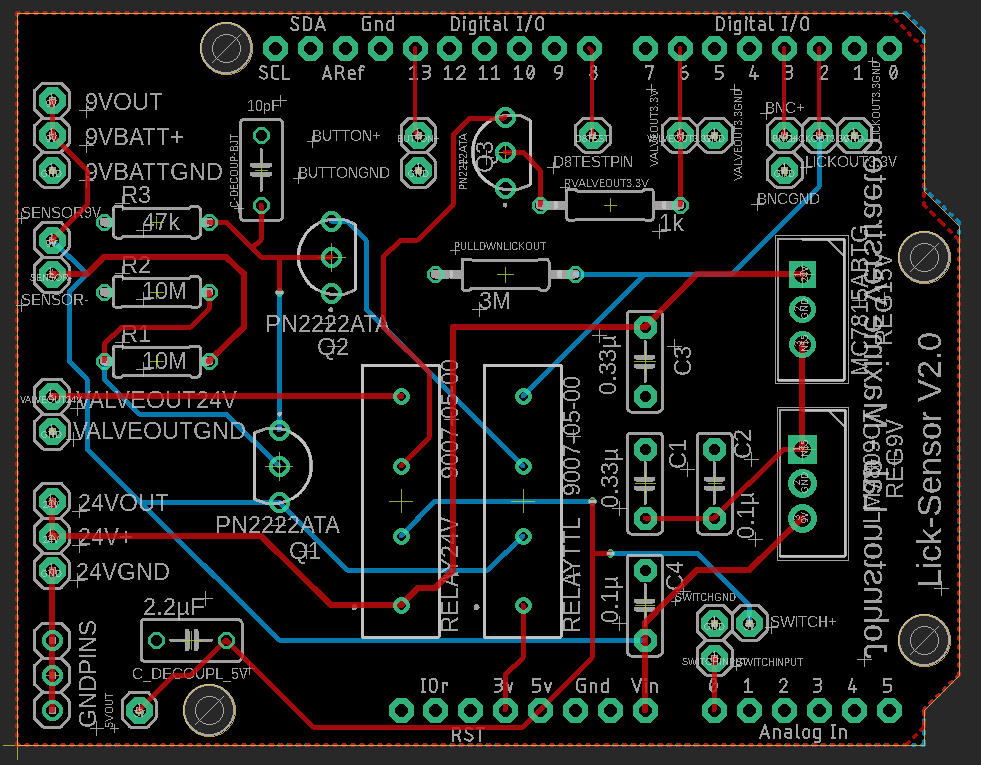
\includegraphics[width = 10cm]{images/schematic.PNG}
    \caption{PCB View}
    \label{fig:schematic}
\end{figure}

\begin{figure}[h!]
    \centering
    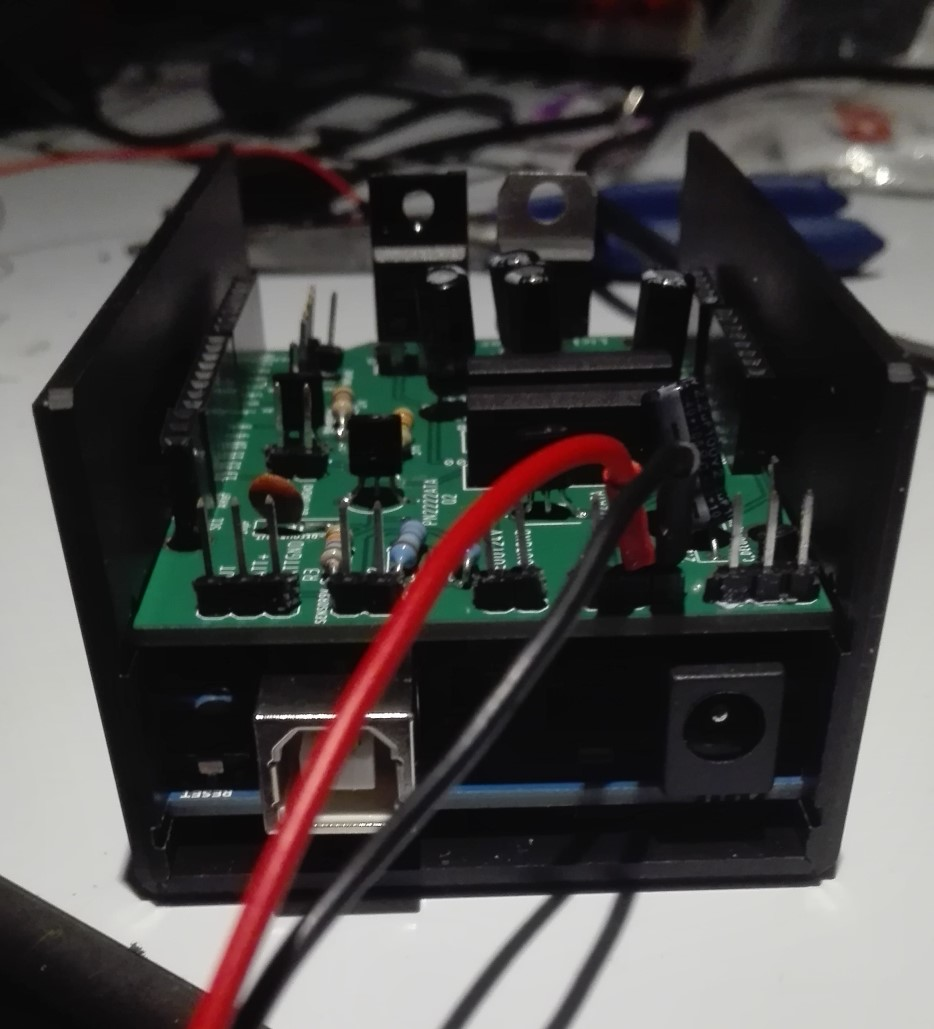
\includegraphics[width=7cm]{images/enclosure.jpg}
    \caption{View of the PCB on top of the Arduino}
    \label{fig:my_label}
\end{figure}

\subsection{Adding a second valve for droplet removal}
For behavioral studies it might be interesting to be able to remove the droplet if it is not licked. To do so, we need to open the circuit to open air to be able to drain the pipe. This therefore requires a second valve.
It is implemented in third version of the design (Section \ref{designV3}).


\section{Troubleshooting}
Note: several ground pins are available on the PCB for easy measurements.
\subsection{The valve doesn't activate}
Make sure that the device is powered by 24V DC.
Check if the valve is opened or closed by putting water in the water tank above.
If it is open check the subsection \ref{staysOpen}.
If it stays closed, check with an oscilloscope if 24V is sent to the valve when push-button is pressed. If it is the case and no water is flowing through, the valve might be blocked due to residues (sugars, ions, ... in the valve). Simply try to apply more pressure to the water (blowing hard on the water syringe might do the trick) to try and unclog it.
\subsection{The valve stays open}
\label{staysOpen}
If the valve is always open, check that the switch on the box is on low position. Indeed, if it is up, the valve will stay open.

If the valve still stays open, check with an oscilloscope if a 24V signal is sent to the valve (you can check the BNC output). If the switch is low, and no button is pressed, the signal should be ground If it stays to 24V no matter what, the reed relay might be broken (fused in closed position). In such cases, the reed relay might need replacement.
Note: ideally, a socket should be placed on the PCB to avoid the need to (un)solder the relay everytime which tends to damage the PCB.
Note2: a new design with another BJT instead of a relay is discussed in section \ref{newPCB}.

\subsection{Push-button/switch doesn't work}
Unscrew the box and check that the wires (2 for the push-button (digital signal pulled up and ground); 3 for the switch (5V, ground, signal)) are still in place both on the button itself and on the PCB pins.
If so, plug the USB into the Arduino and open the Serial monitor. When a button is activated, a corresponding message should appear in the Serial monitor (Note: the Serial should be set to 500000 bauds).

\subsection{Is there a polarity for the sensor?}
One of the sensor is connected to 9V and therefore should not be touching any ground. 
The other sensor is connected to ground through a series of resistors.

\section{Improvements}
\subsection{Zener Diode}
A Zener diode can be used to control the voltage and make sure that no change in sensitivity appears as voltage decreases in case of a battery-powered application. It could also be used as a voltage regulator for the DC Supply.

\subsection{Replacement of the Relay}
The relays have a limited lifetime expectancy, especially in 24V solenoid applications. They can easily be replaced if a socket is present on the PCB. An optocoupler can also be used but are way bigger. 

A new design is proposed in section \ref{newPCB} where the relay is replaced by a FET.

\subsection{Snubber circuit and flyback diode on the valve}
A snubber circuit can be added on the PCB (instead of soldered above) to reduce peak voltage/current and a flyback diode could be added as well.

\subsection{Reduce the current flowing through the mouse}
R1 and R2 could be increased (20M ohms) to reduce current flowing through the subject but reduces reliability.

\subsection{FET instead of BJT ?}
Transistors used in the actual designs are BJT wich are okay in a low current application but FET could probably do, even if the voltage-controlled is less convenient than BJT's current-controlled.
The MOSFETs present high input impedance, less fabrication dispersion, very small, easy to scale.
BJTs present input capacitance (bad for HF), higher output resistance (not suited for low-impedance load), lower gain/stage so SNR quickly degrades, current-operated -> higher consumption

In the end, we could use MOSFET to reduce the consumption but this is not necessary.
Additionaly, FETs are harder to use at logic gate signal (need to use FETs like IRL540 which are more expensive).

\subsection{Avoid shorts with stackable design}
One of the issues I ran into, was that my power pins were spatially close (on top) of the Arduino USB Frame (connected to ground). This may have cause a short-circuit between 24V or 9V and Ground. One solution would be to spatially move those pins in another place.
The other solution which I did was to add one more layer of stackable header to further separate the PCB and the µC. This also allows more air to cool both the PCB and the Arduino down.

\subsection{MTA connectors}
Once the design is tested and validated, we can also implement some MTA connectors instead of the pin headers. This will however increase the cost of the design but it might be interesting if the device is shared to other people.

\subsection{Photobeam detection}
By implementing a photobeam, the animal can signal it is ready for stimulation by approaching the sensor without even licking it. This data can then be used to logically control the water tank valve.

\subsection{Shielded lines}
The solenoid valve may create some noise for othe devices in the lab as well as pick up some noise. Shielded lines can be included if needed.

\subsection{New PCB Design}
\label{newPCB}
A new PCB design is proposed here which replaced the 24V relay by a FET as well as includes some improvements discussed here-above (flyback diode).
The eagle files are available on request and the schematic is shown in section \ref{schematicV2}

\begin{figure}[h!t!b!]
    \centering
    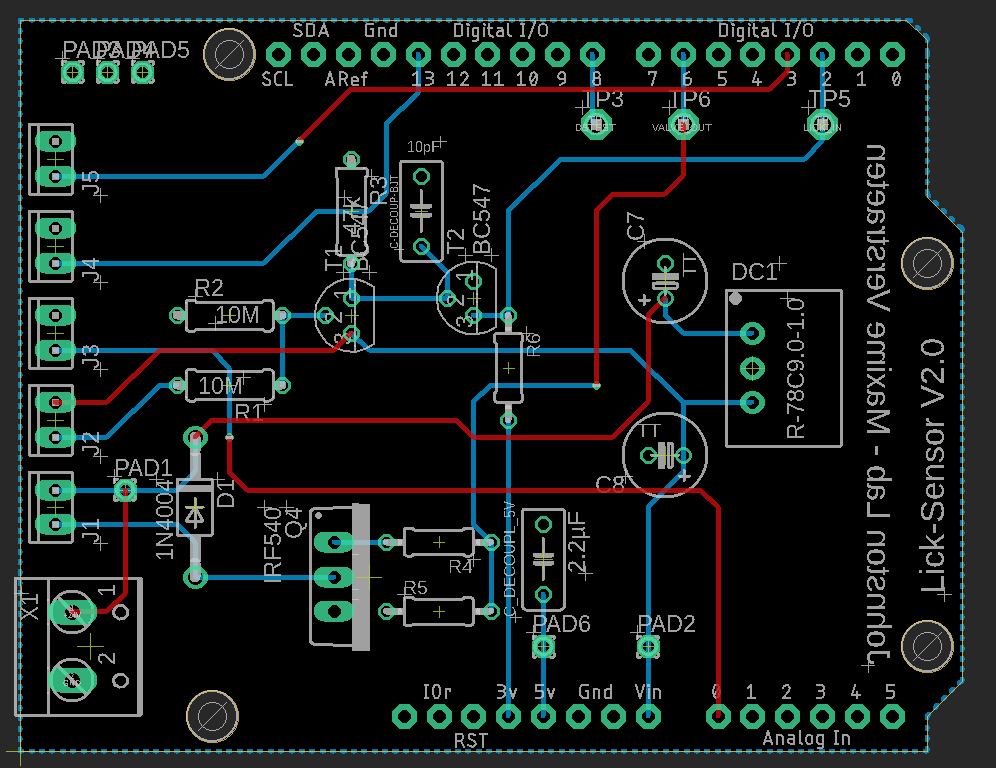
\includegraphics[width = 8cm]{images/schematicV2.PNG}
    \caption{PCB V2}
    \label{fig:PCBV2}
\end{figure}

\subsection{PCB Design V3}
\label{designV3}
To add the new valve and bring some of the improvements discussed here-above, a third version of the PCB has been designed and printed.

This new version does not use reed relays which should increase reliability.



\begin{figure}[h!t!b!]
    \centering
    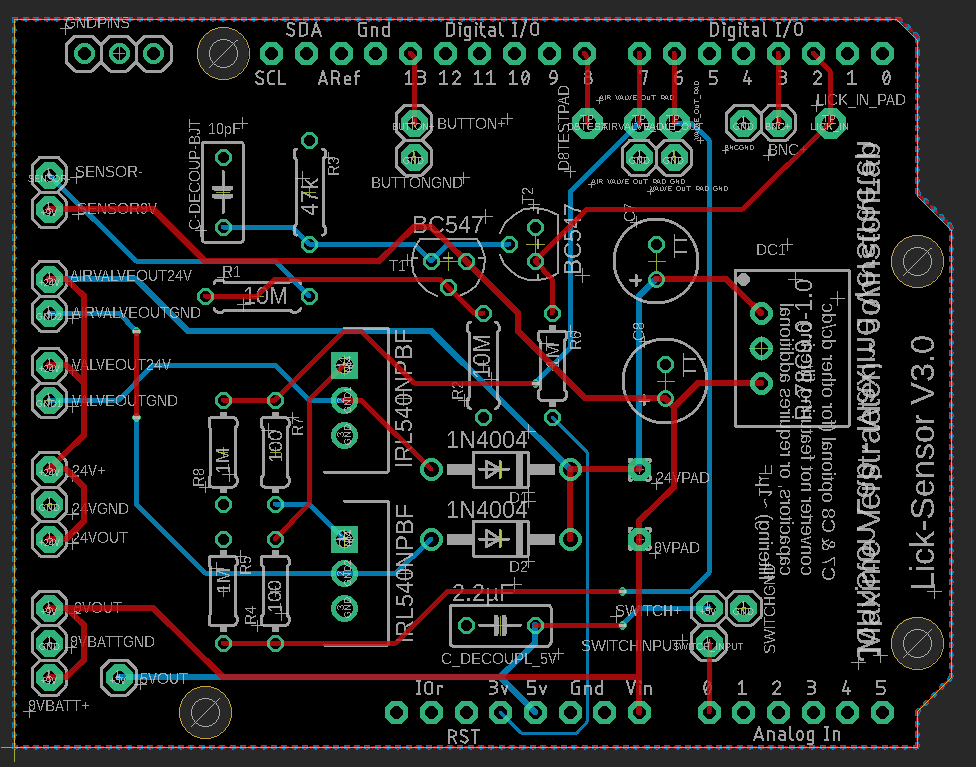
\includegraphics[width = 8cm]{images/BoardViewV3.PNG}
    \caption{PCB V3}
    \label{fig:PCBV3}
\end{figure}


\appendix
\section{Power dissipation by linear voltage regulators}
The first design used linear voltage regulators to transform the 24V to 9V able to power the Arduino.
They transform excessive voltage in heat.
Therefore the power dissipated = ((24V-15V)+(15V-9V))*Imax
Imax =  1.095V/20ohms (current measurement with voltage meter) = 55mA.

Safety measure : 100mA.

So we get power dissipated = 1.5W
Or 900mW for the first regulator and 600mW for the second one.
The regulators comes within a TO-220 package which is fine for under 1W of dissipation (rule of thumb). However, in a closed box, there will be no airflow.

The datasheet of the regulators specify 60°C/W as thermal resistance for junction/ambient.

\begin{figure}[h!]
    \centering
    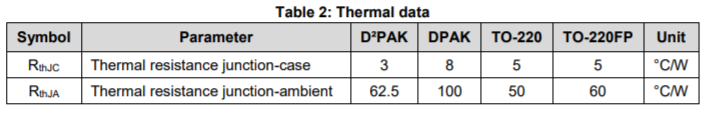
\includegraphics[width = 10cm]{images/thermalData.png}
    \caption{Thermal Data}
    \label{fig:thermalData}
\end{figure}

So at 900mW it's 54°C above ambient. Worst case ambient would be 40°C room temp + enclosed box.. Estimates about 60°C. That makes a total of 104°C.

The datasheet mentions that the maximum operation temperature is 125°C. So we're just under.


\begin{figure}[h!]
    \centering
    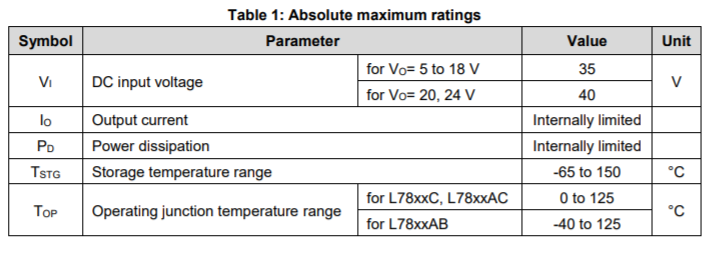
\includegraphics[width = 10cm]{images/thermalData2.png}
    \caption{Maximum operating temperature}
    \label{fig:thermalData2}
\end{figure}

The idea was therefore to drill some holes for the air to flow through the box and monitor the temperature. If it rose too high, a fan was to be added (required 9V and 5V pins were already present on the PCB).

On the PCB: I obtained 1.130V/20ohms = 57mA, as expected.

A simpler and more reliable solution (as the device is used with other devices around, for long term use, by people without skills in electronics) was to replace the linear regulators by DC/DC switching regulators, way more efficient but more expensive.

\newpage

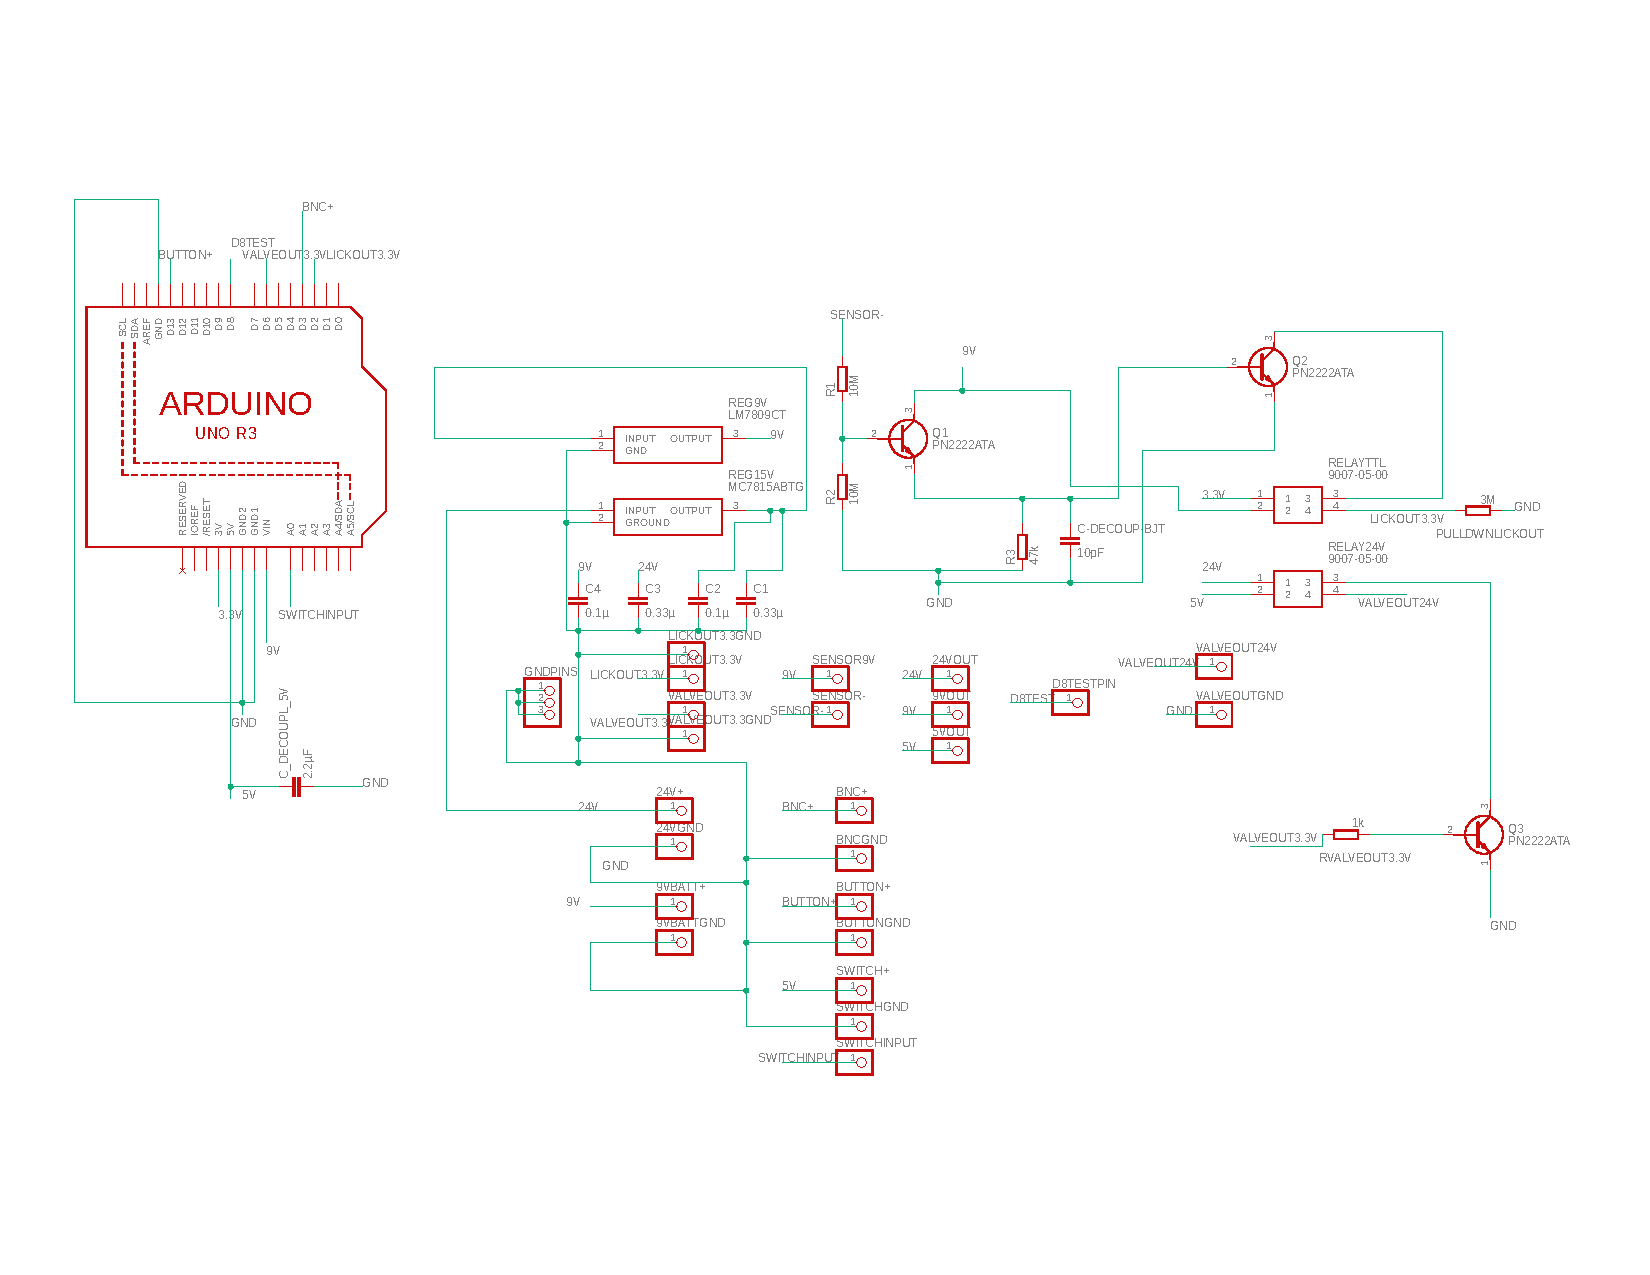
\includepdf[pagecommand= \section{PCB Schematic \label{schematic}}, scale = 1, angle = 270]{images/schematic}


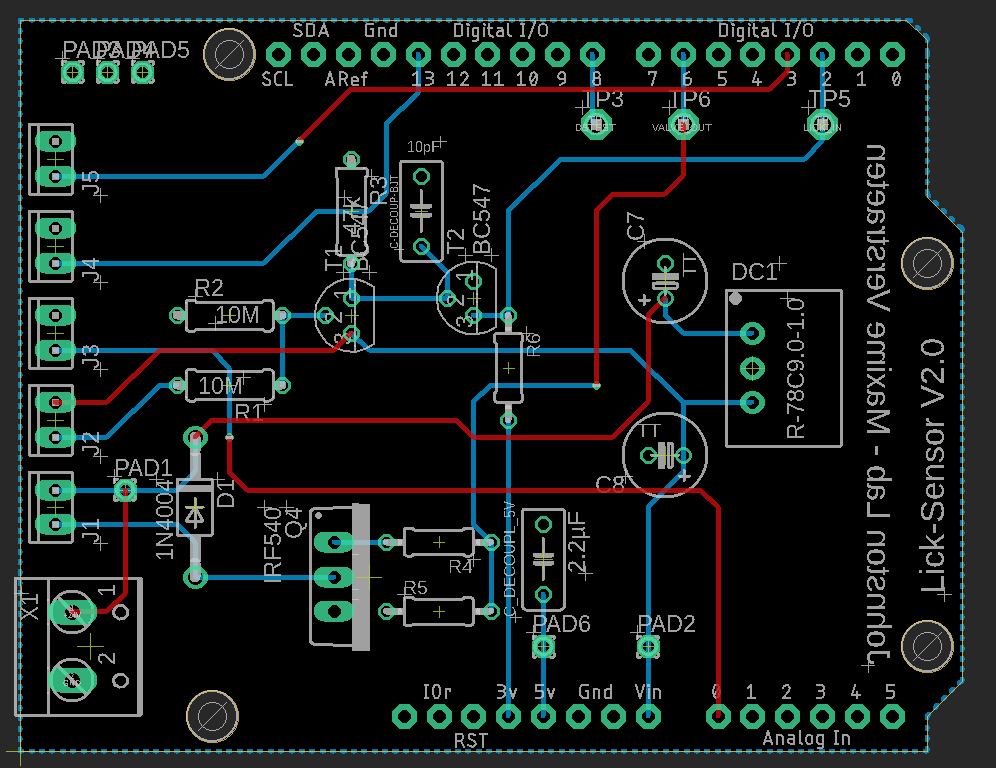
\includepdf[pagecommand= \section{PCB Schematic v2\label{schematicV2}},scale = 1,angle = 270, ]{images/schematicV2}



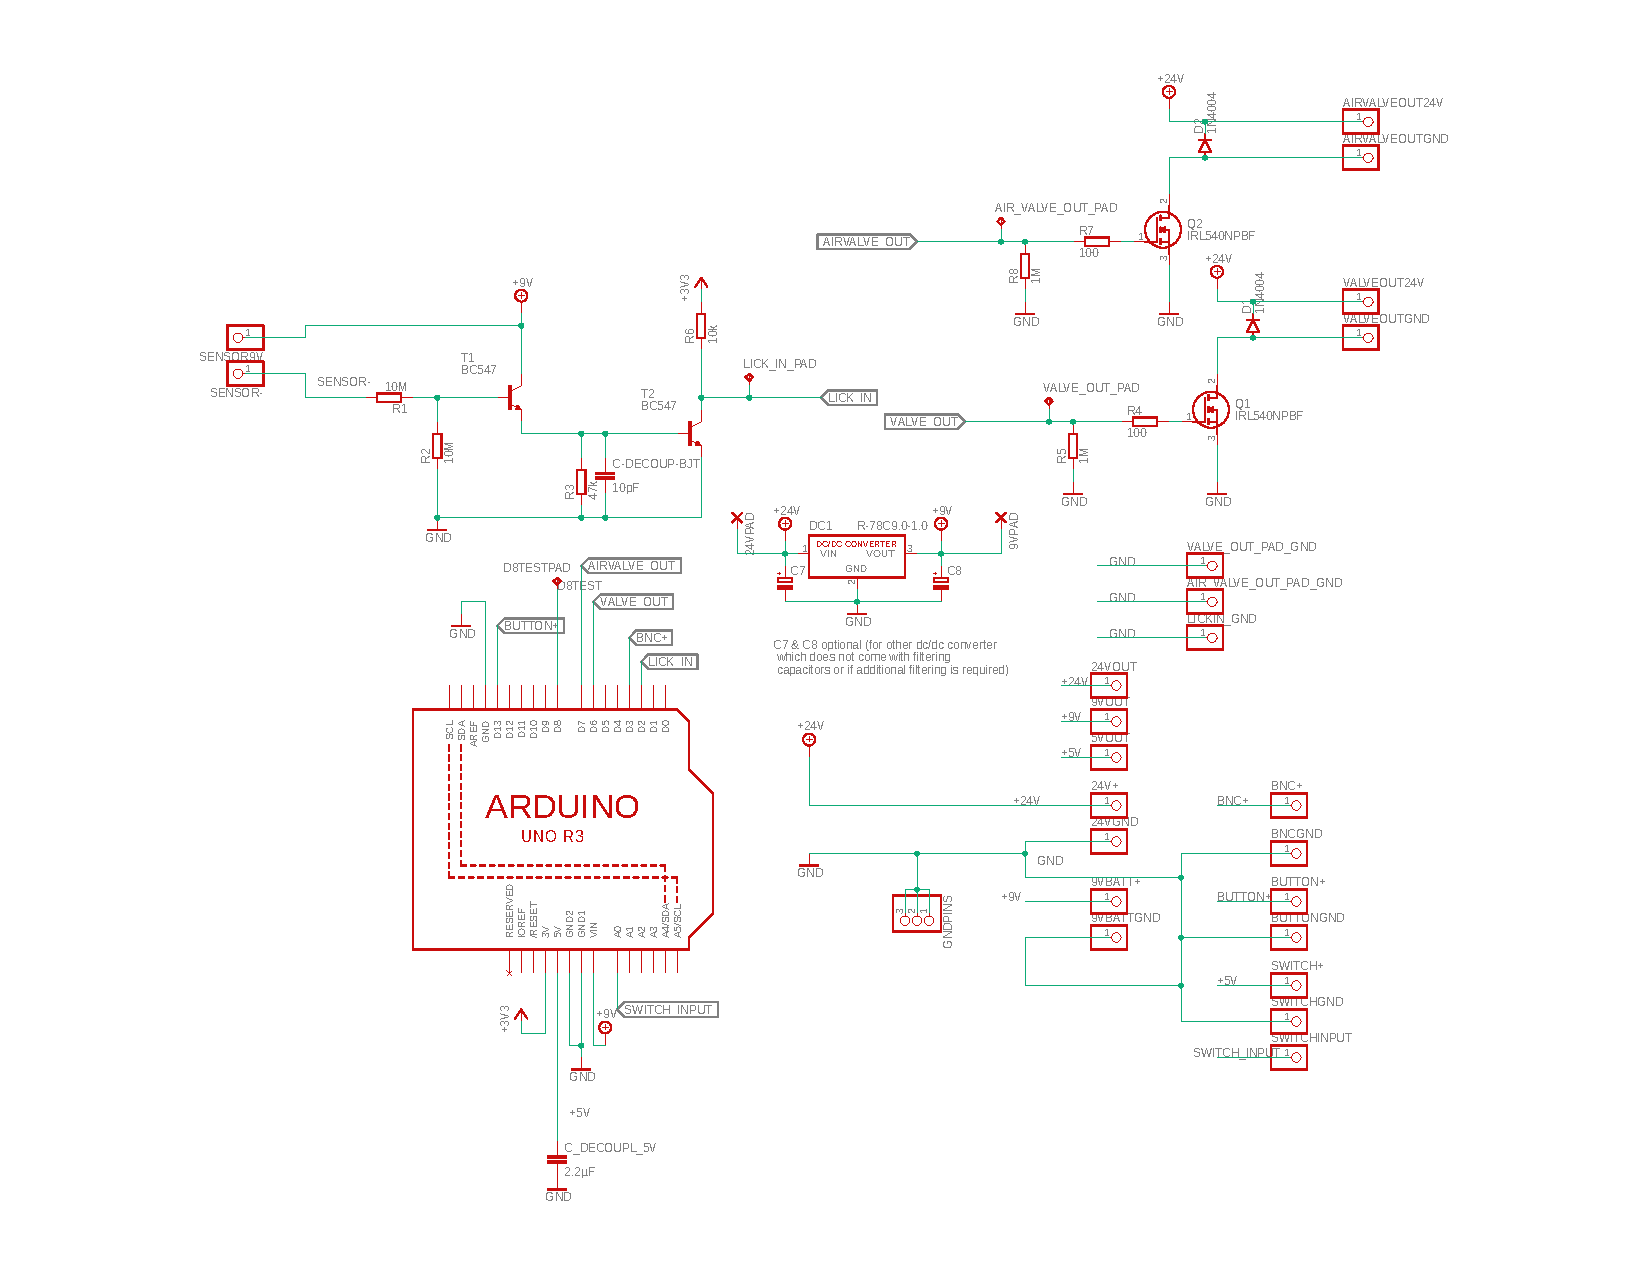
\includepdf[pagecommand= \section{PCB Schematic v3\label{schematicV3}},scale = 1,angle = 270, ]{images/schematicV3}

\bibliographystyle{alpha}
\bibliography{biblio}

\end{document}